\documentclass{beamer}
\usepackage{fancybox}
\usepackage{tikz}
\usetikzlibrary{arrows.meta,
                chains,
                positioning, 
                shadows.blur, shapes.arrows}
              
\usetheme{Madrid}

\title{Neuro-symbolic AI}
\author{Robert Hoehndorf}
\date{\today}

\begin{document}

\frame{\titlepage}

\begin{frame}
\frametitle{Organization}
\begin{itemize}
\item New room: B9-3222
\item New time: 14:30-17:30 (or: 2:30pm to 5:30pm)
\end{itemize}
\end{frame}

\begin{frame}
\frametitle{Organization}
\begin{itemize}
\item Starting next week: we {\em all} read and discuss papers
  \begin{itemize}
  \item list is online (Zotero Group)
    \begin{itemize}
    \item \url{https://www.zotero.org/groups/5368923/cs394y_kaust_neurosymbolic_ai/library}
    \end{itemize}
  \item welcome to add your own (just join the group)
  \item each week: 2-4 papers
  \item mix of: Foundations + Theory, Applications
  \item we all read the papers
  \item 1-2 presenters, overview of the paper, leading discussion
  \end{itemize}
\end{itemize}
\end{frame}


\begin{frame}
  \frametitle{Motivation}
  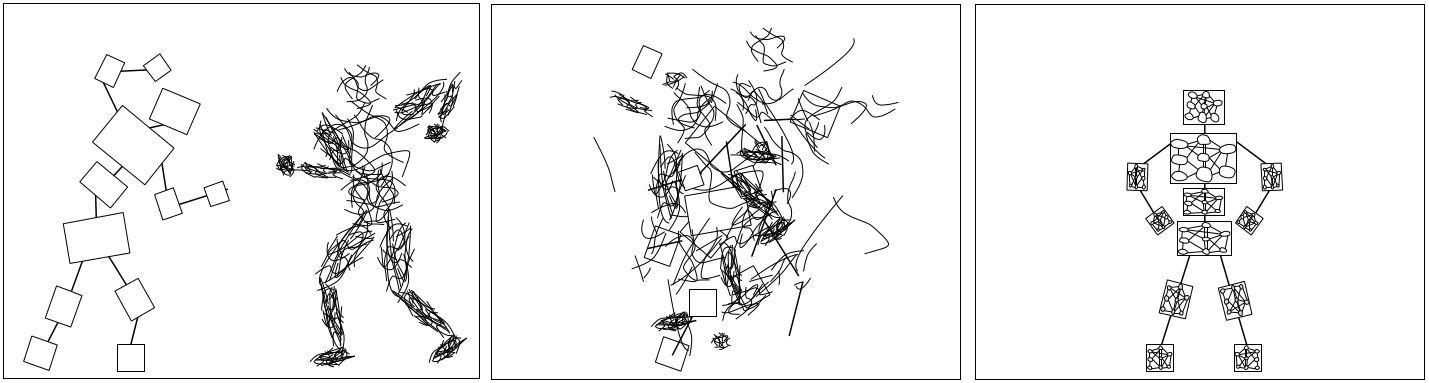
\includegraphics[width=\textwidth]{minsky-figure.png}
\end{frame}

% Limitations of Learning and Reasoning Systems
\begin{frame}
\frametitle{Limitations of Learning and Reasoning Systems}
\begin{itemize}
\item Learning Systems: Data hungry, limited transfer, brittle,
  opaque, no use of prior knowledge
\item Symbolic Reasoning Systems: Brittle, limited scope,
  combinatorial explosions
  \pause
\item The limitations of each approach are largely {\em
    complementary}!
\end{itemize}
\end{frame}

% Complementarity of Techniques
\begin{frame}
\frametitle{Complementarity of Techniques}
\begin{itemize}
\item Statistical learning successful in pattern recognition
\item Symbolic reasoning effective in planning and diagnosis
\end{itemize}
\end{frame}

% Task-Based Distinction
\begin{frame}
\frametitle{Task-Based Distinction}
\begin{itemize}
\item Deduction vs. Induction vs Abduction:
  \begin{itemize}
  \item Classical distinction between reasoning and learning and diagnosis/explanation
  \end{itemize}
\item Compression vs. Decompression:
  \begin{itemize}
  \item Learning as compression
  \item reasoning as decompression
  \end{itemize}
\end{itemize}
\end{frame}

\begin{frame}
  \frametitle{Deduction vs induction vs abduction}
  \begin{itemize}
  \item Deduction: Given a set of formulas $T$ and a specific
    deductive calculus $\vdash$, derive the specific conclusion
    $\phi$
    \pause
  \item Induction: Given a set of specific observations
    $\phi_1,...,\phi_n$, find $T$ such that $T \vdash \phi_i$ for all
    $1 \leq i \leq n$
    \pause
  \item Abduction: Given a set of statements $T$, a specific
    observation $\phi$, and a specific deductive calculus $\vdash$,
    find a statement $\psi$ such that
    $T \cup \{ \psi \} \vdash \phi$
  \end{itemize}
\end{frame}

\begin{frame}
  \frametitle{Compression and decompression}
  \begin{itemize}
  \item Learning as compression: ``compress'' observations
    $\phi_1,...,\phi_n$ into a smaller model $T$
    \begin{itemize}
    \item using any kind of regularity in the data to compress
    \end{itemize}
  \item Reasoning as decompression: produce ``prediction'' $\phi$ from
    model $T$
    \begin{itemize}
    \item $\phi$ was already implicit in $T$
    \item reasoning/deduction to make it explicit
    \end{itemize}
  \end{itemize}
\end{frame}

% Representation-Based Distinction
\begin{frame}
\frametitle{Representation-Based Distinction}
\begin{itemize}
\item ``Model-Free'' Representations: Predominant in learning systems
\item ``Model-Based'' Representations: Typical in reasoning systems.
\item Properties: Compositional, referential, homologous,
  interpretable, symbolic, discrete
\end{itemize}
\end{frame}

\begin{frame}
  \frametitle{Taxonomy of neuro-symbolic systems (Kautz, AAAI 2020)}
  \begin{itemize}
  \item symbolic Neuro symbolic
  \item Symbolic[Neuro]
  \item Neuro;Symbolic
  \item Neuro:Symbolic $\rightarrow$ Neuro
  \item Neuro$_{symbolic}$
  \item Neuro[Symbolic]
  \end{itemize}
\end{frame}

\begin{frame}
  \frametitle{symbolic Neuro symbolic}
  \centering
  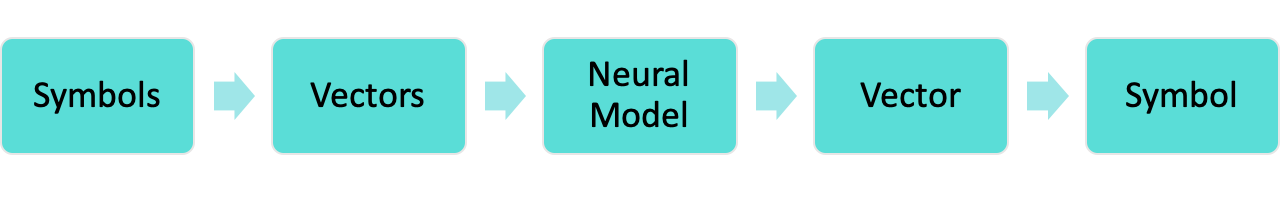
\includegraphics[width=.7\textwidth]{ns10.png}
  \begin{itemize}
  \item symbols as input and output
  \end{itemize}
  % basic pattern above; most NLP is this type
\end{frame}

\begin{frame}
  \frametitle{Symbolic[Neuro]}
  \centering
  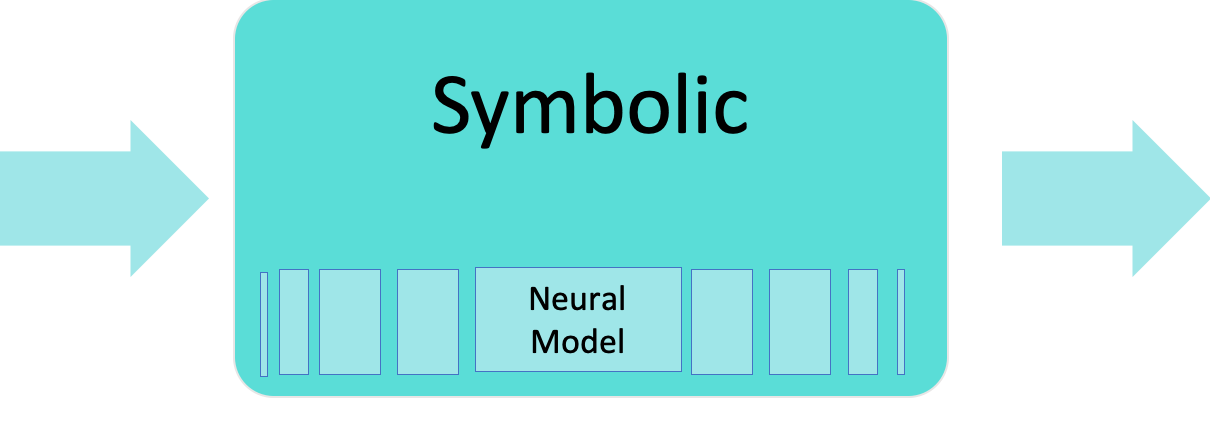
\includegraphics[width=.7\textwidth]{ns11.png}
  \begin{itemize}
  \item symbolic solver, use neural model internally
    % \begin{itemize}
    % \item e.g., search strategy
    % \end{itemize}
  \end{itemize}
  % reinforcement learning for search for proof
  % AlphaGO
\end{frame}

\begin{frame}
  \frametitle{Neuro; Symbolic}
  \centering
  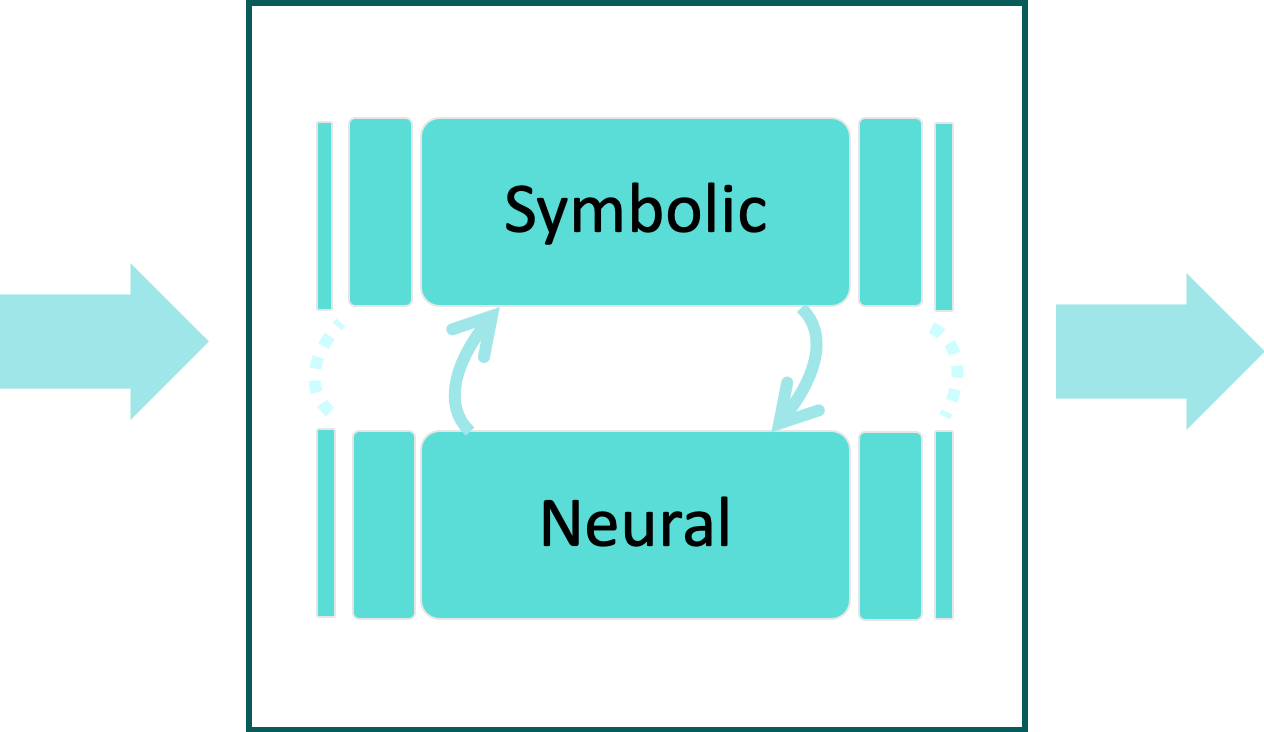
\includegraphics[width=.7\textwidth]{ns12.png}
  \begin{itemize}
  \item symbols from data, then reason
  \end{itemize}
\end{frame}

\begin{frame}
  \frametitle{Neuro:Symbolic $\rightarrow$ Neuro}
  \centering
  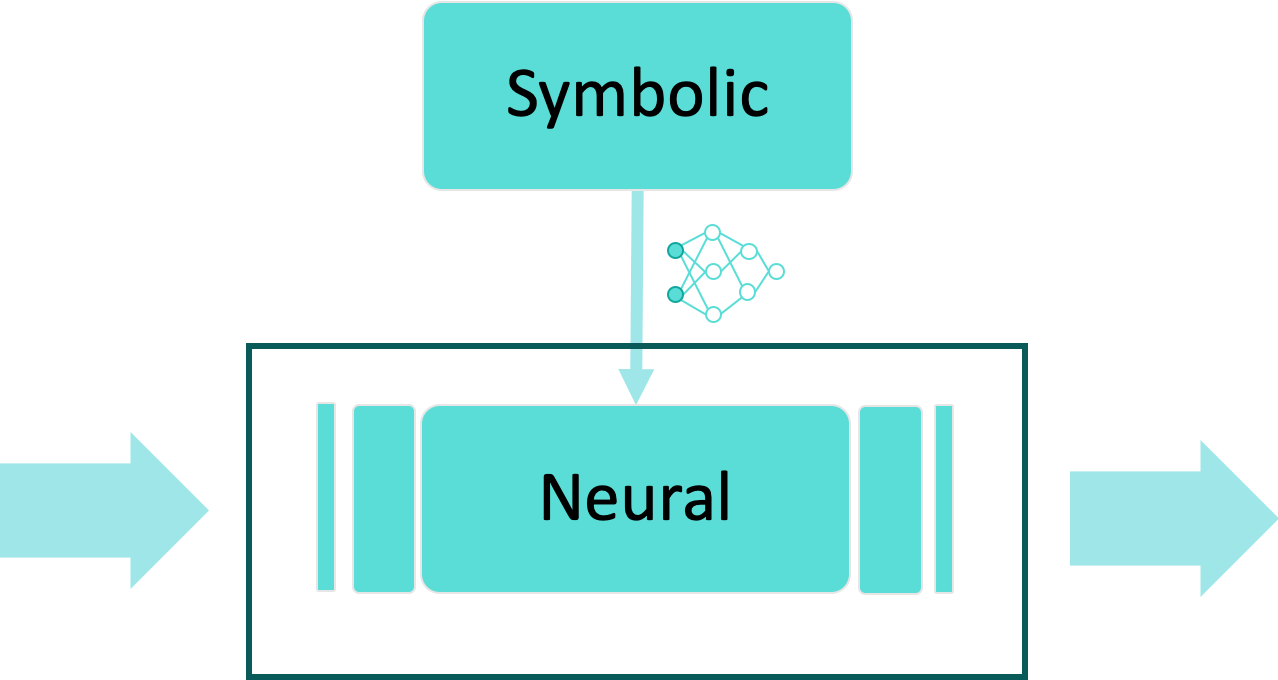
\includegraphics[width=.7\textwidth]{ns13.png}
  \begin{itemize}
  \item symbolic knowledge translated into neural model structure
  \end{itemize}
\end{frame}

\begin{frame}
  \frametitle{Neuro$_{symbolic}$}
  \centering
  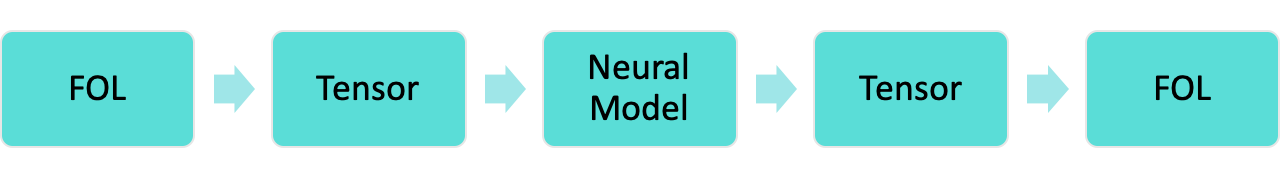
\includegraphics[width=.7\textwidth]{ns14.png}
  \begin{itemize}
  \item symbolic manipulation as neural operations
    % Pattern 7, learning with prior knowledge
  \end{itemize}
\end{frame}

\begin{frame}
  \frametitle{Neuro[Symbolic]}
  \centering
  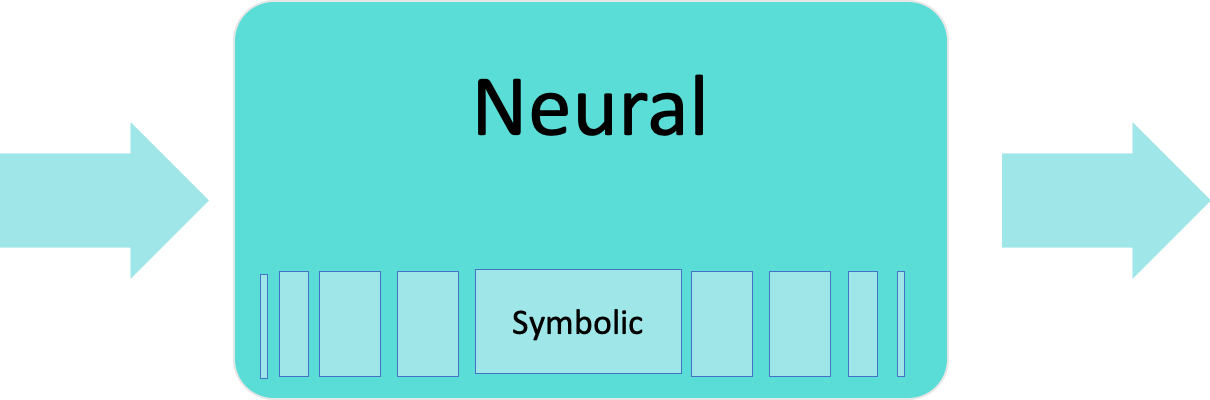
\includegraphics[width=.7\textwidth]{ns15.png}
  \begin{itemize}
  \item learning relation between symbols
  \item attention on particular symbols
    % This is basically what GNNs do (?)
  \end{itemize}
\end{frame}

% Design Patterns and Notation
\begin{frame}
\frametitle{Design Patterns and Notation}
\begin{itemize}
\item Design patterns: General reusable solutions, e.g., in software
  design
\item Hierarchical taxonomy and graphical notation
\item Examples: Software Engineering (Design Patterns), Knowledge
  Engineering (CommonKADS), Ontology Engineering
\item Here: a ``boxology'' introduced by Frank van Harmelen and
  Annette ten Teije
  \begin{itemize}
  \item boxes and arrows
  \item no semantics
  \end{itemize}
\end{itemize}
\end{frame}

\begin{frame}
  \frametitle{Design Patterns and Notation}
  \begin{itemize}
  \item oval nodes: algorithmic components
    \begin{itemize}
    \item deduction: \Ovalbox{KR}
    \item learning: \Ovalbox{ML}
    \end{itemize}
  \item rectangular nodes: inputs, outputs
    \begin{itemize}
    \item model-based, symbolic, relational structures: \fbox{sym}
    \item model-free: \fbox{data}
    \end{itemize}
  \item maybe special node for ``model''
  \end{itemize}
\end{frame}

\begin{frame}
  \frametitle{Design Patterns and Notation}
  \begin{itemize}
  \item \fbox{sym} boxes are inputs and outputs of (traditional) KR
    reasoning systems:
    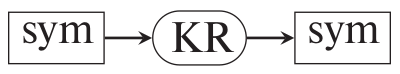
\includegraphics[width=.25\textwidth]{ns1.png}
  \item \fbox{data} boxes are inputs and outputs of (traditional)
    machine learning systems:
    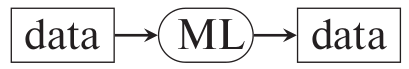
\includegraphics[width=.25\textwidth]{ns2.png}
  \end{itemize}
\end{frame}

\begin{frame}
  \frametitle{Generating models}
  \centering
  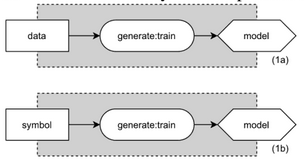
\includegraphics[width=.5\textwidth]{ns3.png}
\end{frame}

\begin{frame}
  \frametitle{Inference}
  \centering
  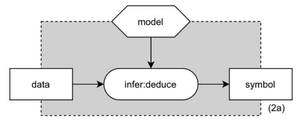
\includegraphics[width=.5\textwidth]{ns4.png}
  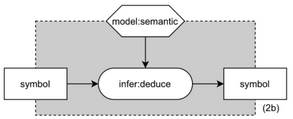
\includegraphics[width=.5\textwidth]{ns5.png}
\end{frame}

\begin{frame}
  \frametitle{Machine learning workflow}
  \centering
  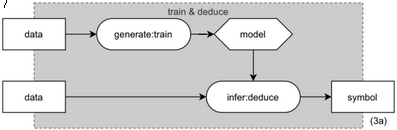
\includegraphics[width=.7\textwidth]{ns6.png}
\end{frame}


\begin{frame}
  \frametitle{Hybrid systems}
  \centering
  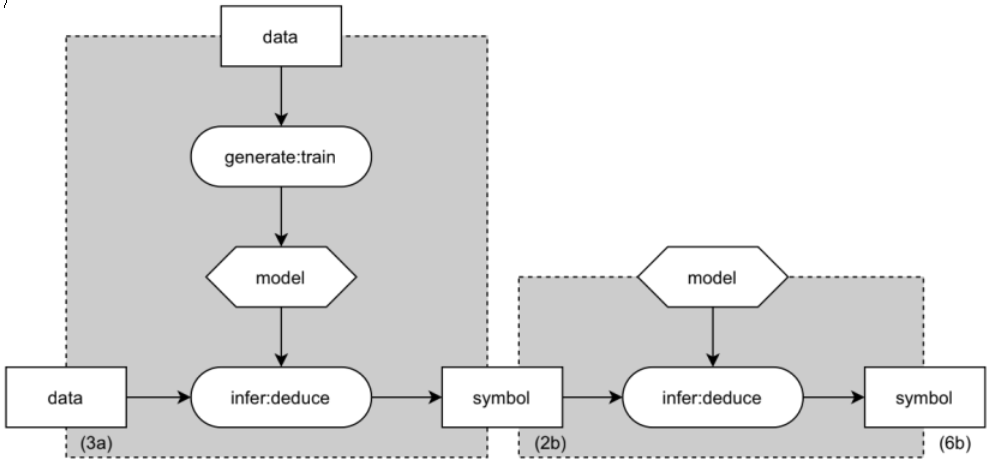
\includegraphics[width=.7\textwidth]{ns7.png}
  % AlphaGO
\end{frame}

\begin{frame}
  \frametitle{Learning an intermediate representation}
  \centering
  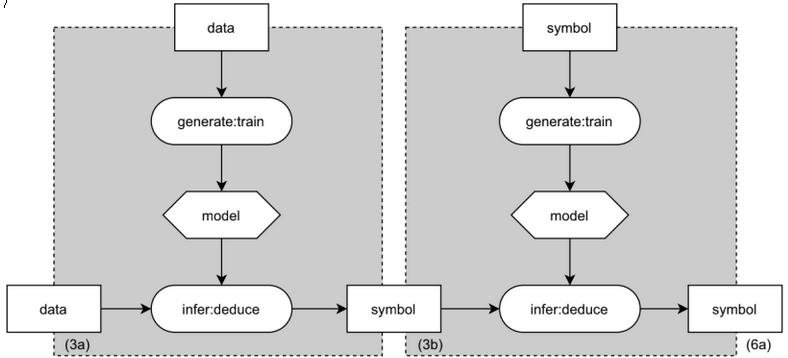
\includegraphics[width=.7\textwidth]{ns8.png}
  % DeepProbLog
  % DeepMind's Atari experiment
\end{frame}

\begin{frame}
  \frametitle{Learning with prior knowledge}
  \centering
  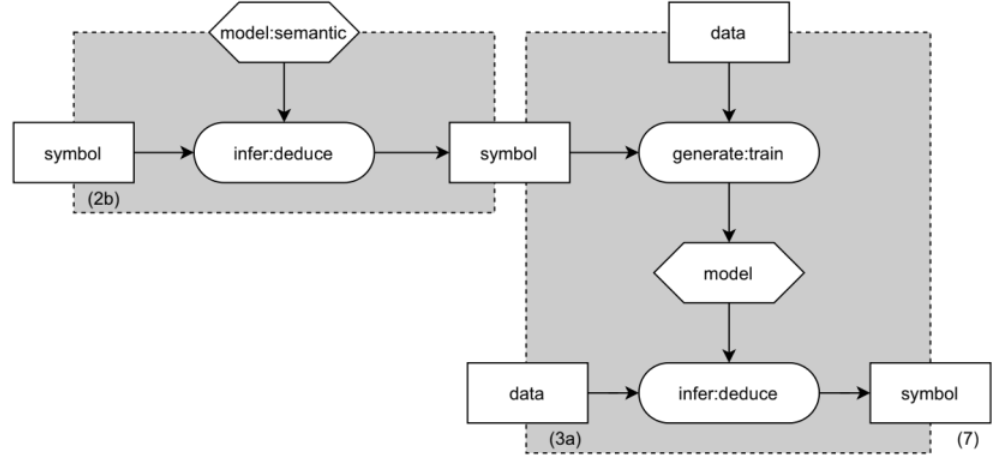
\includegraphics[width=.7\textwidth]{ns9.png}
  % knowledge graphs/bases as symbolic prior
  % semantic loss function (degree to which symbolic knowledge is
  % violated)
\end{frame}

\begin{frame}
  \frametitle{Explanation}
  \centering
  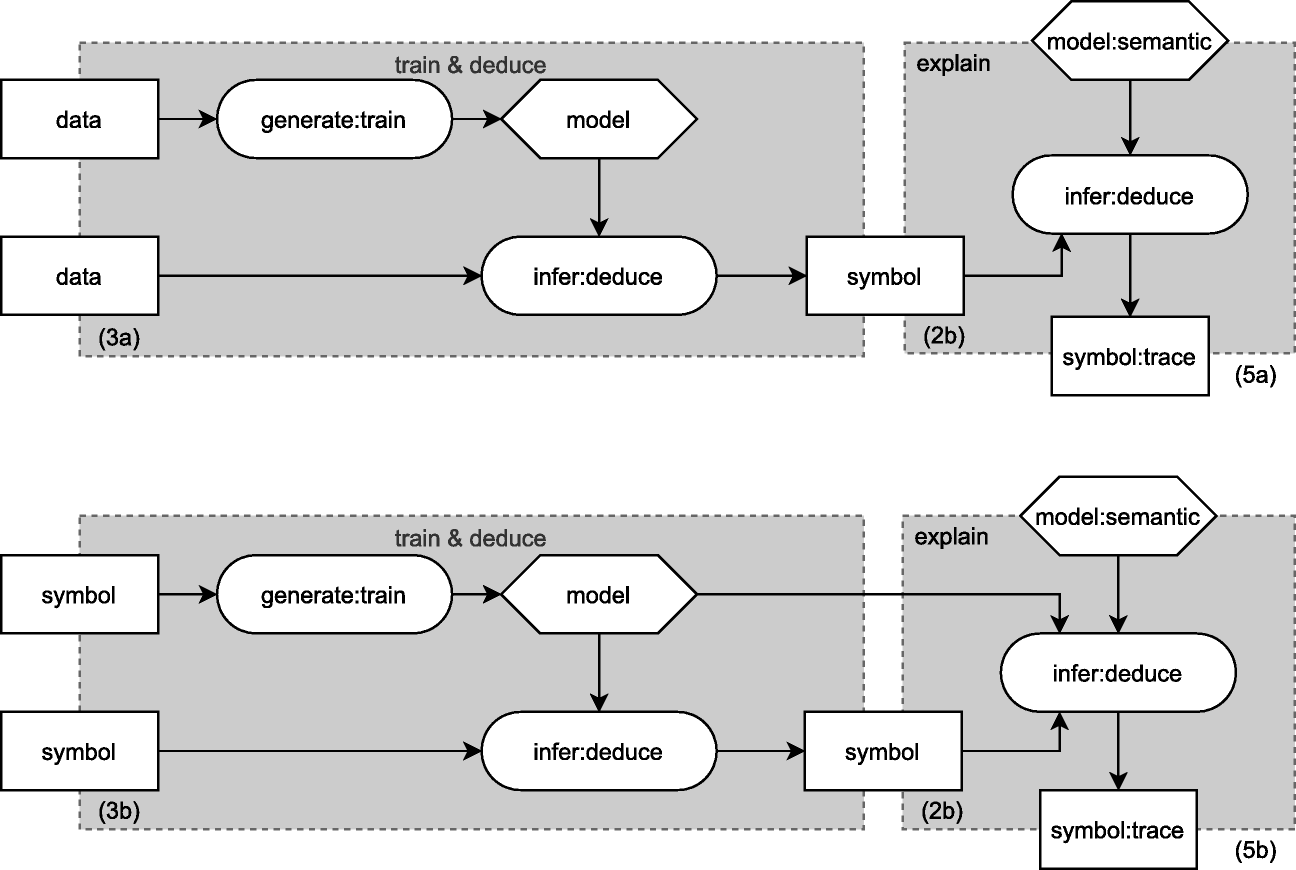
\includegraphics[width=.7\textwidth]{im1.png}
\end{frame}

\begin{frame}
  \frametitle{Learning to reason}
  \centering
  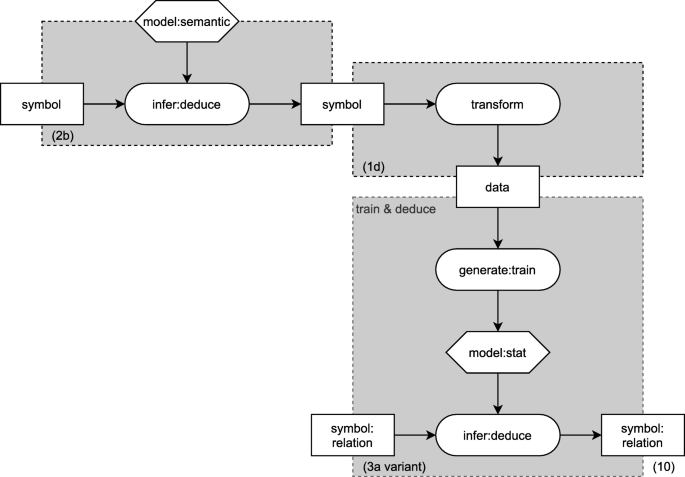
\includegraphics[width=.7\textwidth]{im2.png}
\end{frame}

\begin{frame}
  \frametitle{Other dimensions (Raedt et al., 2020)}
  \begin{itemize}
  \item directed vs un-directed models
  \item model-theoretic vs. proof-theoretic inference
  \item Logic vs. Neural
  \item Boolean vs. probabilistic semantics
  \item Structure vs. parameter learning
  \item Symbols vs. Sub-symbols
  \item Type of Logic
  \end{itemize}
\end{frame}

\begin{frame}
  \frametitle{Other dimensions}
  \centering
  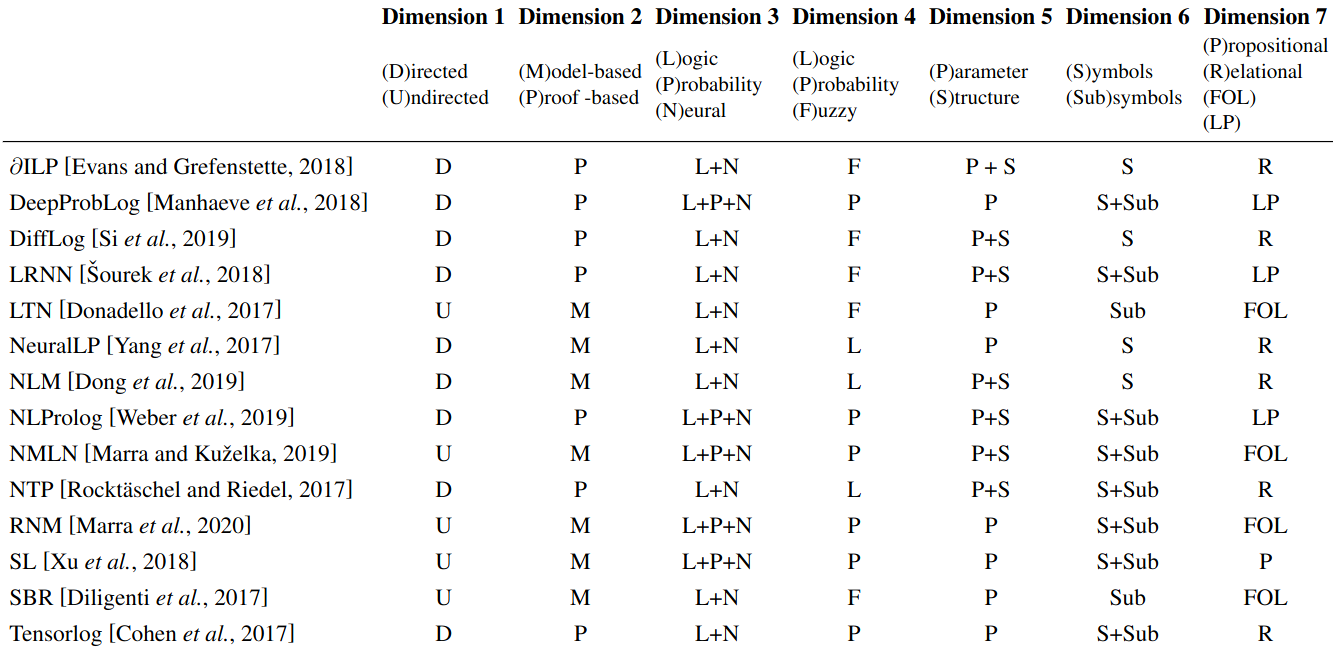
\includegraphics[width=1\textwidth]{im3.png}
\end{frame}

\begin{frame}
  \frametitle{Applications of Neuro-Symbolic methods}
  \begin{itemize}
  \item Solve much harder problems
    \begin{itemize}
    \item few shot, zero shot
    \item deduction
    \end{itemize}
  \item Learn with dramatically less data, ultimately for a large
    number of tasks rather than one narrow task
  \item Provide inherently understandable and controllable decisions
    and actions
  \end{itemize}
\end{frame}

\end{document}

% Introduction:

% Minsky's paper

% http://arxiv.org/abs/1905.12389

% http://arxiv.org/abs/2305.08876

% http://arxiv.org/abs/2302.02093




% From knowledge graph to knowledge base completion


% Neural logical query answering

%%% Local Variables:
%%% mode: latex
%%% coding: utf-8
%%% TeX-master: t
%%% eval: (TeX-run-style-hooks "beamer")
%%% End:
